../cictikz/src/cictikz/data/tex/cictikz_preamble.tex

% Moore state machine: the output combinatorics see only the state, so
% the output only changes on clock edges.

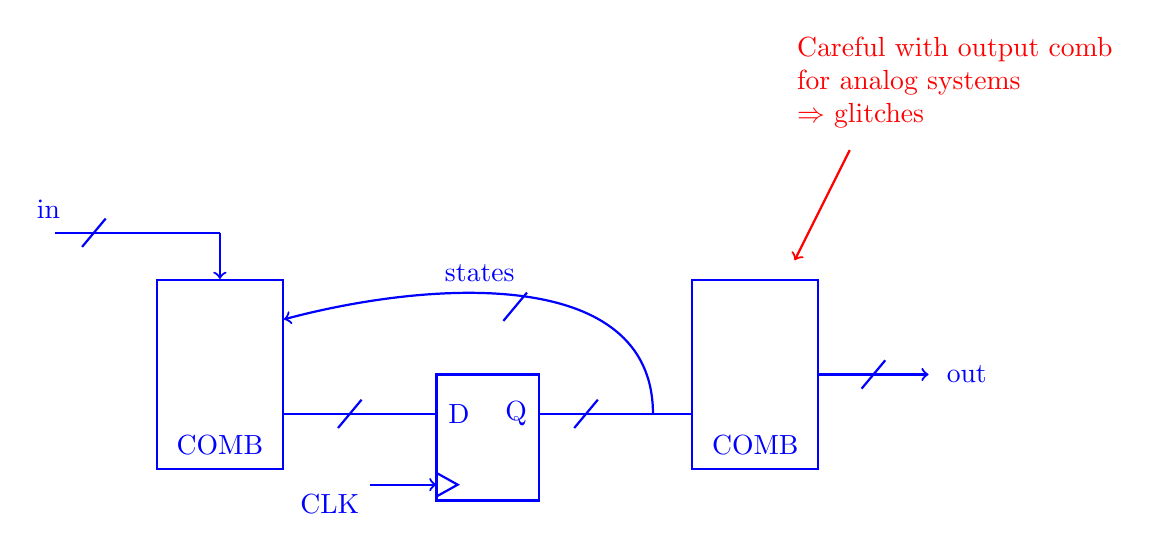
\begin{tikzpicture}[thick, color=blue,
  blk/.style={draw=blue, rectangle, minimum width=1.6cm, minimum height=2.4cm},
  bs/.style={},
  a/.style={->}]

  % combinatorial blocks and flip-flop
  \node[blk] (c1) at (0,0.3) {};
  \node[anchor=south] at ([yshift=2pt]c1.south) {COMB};
  \node[blk] (c2) at (6.8,0.3) {};
  \node[anchor=south] at ([yshift=2pt]c2.south) {COMB};
  \node[draw=blue, rectangle, minimum width=1.3cm, minimum height=1.6cm]
    (ff) at (3.4,-0.5) {};
  \node[anchor=west] at ([xshift=1pt,yshift=0.3cm]ff.west) {D};
  \node[anchor=east] at ([xshift=-1pt,yshift=0.3cm]ff.east) {Q};

  % clock wedge and CLK wire
  \draw (2.75,-0.95) -- (3.02,-1.1) -- (2.75,-1.25);
  \draw[a] (1.9,-1.1) -- (2.75,-1.1);
  \node[anchor=east] at (1.9,-1.35) {CLK};

  % input bus: feeds only the first COMB (that is what makes it Moore)
  \node[anchor=south east] at (-1.9,2.15) {in};
  \draw (-2.1,2.1) -- (0,2.1);
  \draw[a] (0,2.1) -- (c1.north);
  \draw (-1.75,1.92) -- (-1.45,2.28);   % bus slash

  % COMB -> D
  \draw ([yshift=-0.5cm]c1.east) -- (2.75,-0.2);
  \draw (1.5,-0.38) -- (1.8,-0.02);     % bus slash

  % Q -> output COMB
  \draw (4.05,-0.2) -- ([yshift=-0.5cm]c2.west);
  \draw (4.5,-0.38) -- (4.8,-0.02);     % bus slash

  % states feedback from Q back to the first COMB
  \draw[a] (5.5,-0.2) to[out=90, in=15] ([yshift=0.7cm]c1.east);
  \node[anchor=south] at (3.3,1.35) {states};
  \draw (3.6,0.98) -- (3.9,1.34);       % bus slash

  % output bus
  \draw[a] (c2.east) -- (9.0,0.3);
  \node[anchor=west] at (9.1,0.3) {out};
  \draw (8.15,0.12) -- (8.45,0.48);     % bus slash

  % warning note
  \node[red, align=left, anchor=south west] at (7.2,3.3)
    {Careful with output comb\\for analog systems\\$\Rightarrow$ glitches};
  \draw[red, a] (8.0,3.15) -- (7.3,1.75);

\end{tikzpicture}
\end{document}
